\section{Theoretical foundations}
\label{sec:Theorie}
\subsection{Cosmic radiation}

Charged cosmic radiation mainly consists of high-energy protons, helium and heavy nuclei.
The exact composition depends on the energy level of the particles.
Energies up to $10^{20} \si{\electronvolt}$ can be achieved by that kind of radiation which follows approximately the power law of
\begin{equation*}
  \frac{\symup{d}\Phi}{\symup{d}E} = \Phi_0 E^{\gamma}.
\end{equation*}
Here $\gamma \approx -2.7$ is the spectral index for charged particles.

The IceCube experiment studies muons and neutrinos from atmospherical and astrophysical sources.
Atmospherical particles can be separated into two categories: conventional and prompt muons and neutrinos.
Conventional muons and neutrinos originate from pion and kaon decays in the atmosphere.
Since pions and kaons have a relatively long lifetime, they are losing a part of their energy before decaying into muons and neutrinos.
This results a shift of the energy spectrum from $\propto E^{-2.7}$ to $\propto E^{-3.7}$.
Besides kaons and pions there is also a production of $D$ mesons and $\Lambda_c$ baryons for high energy interactions.
These particles have a very short lifetime, so they are decaying before deposing a relevant amount of energy.
This results to the production of prompt muons and neutrinos with an unshifted energy spectrum of $\propto E^{-2.7}$.
Astrophysical neutrinos are emitted from hadron accelerating sources that are also emitting high energy photons.
These photons are not able to pass dust clouds or other optically dense media.
Neutrinos on the other side have such a small cross-section that they are not interacting with these kind of boundaries.
Assuming shock acceleration \cite{Fermi} is getting a spectral index of $\gamma \approx -2$ for astrophysical neutrinos.

\subsection{The IceCube experiment}
The IceCube experiment is located at the geographical southpole $\SI{1450}{\meter}$-$\SI{2450}{\meter}$ under the ice surface.
Its main purpose is to detect high energy neutrinos and muons.
The detector consists of 86 wires with a total of 5160 photomultipliers (PMT).
These PMTs are detecting Cherenkov radiation resulting from high energy charged particles that are traveling with a velocity greater than the speed of light in that medium.
The speed of light in a medium is given by
\begin{equation}
  c = \frac{c_0}{n}
\end{equation}
where $c_0$ is the vacuum speed of light and $n$ is the refractive index.

7 wires with a bigger PMT density and a smaller distance to each other are located in the center of the detector and form the low energy expansion DeepCore \cite{DeepCore}.
The lower distances and the higher energy efficiency are resulting in a relatively low energy threshold of $\SI{10}{\giga\electronvolt}$.
The rest of the wires that surround DeepCore are forming the In-Ice-Array, the biggest part of the detector.
Since the distances between the PMTs are bigger than in DeepCore, the energy threshold has a value of $\SI{100}{\giga\electronvolt}$.
The air shower experiment IceTop is located on the surface \cite{IceTop}.
The Cherenkov radiation on this part of the experiment is measured in ice tanks.
IceTop serves to study cosmic radiation as well as a veto for the In-Ice-Array.
A schematic representation of the IceCube experiment is shown in figure \ref{fig:cube}.

\begin{figure}
  \centering
  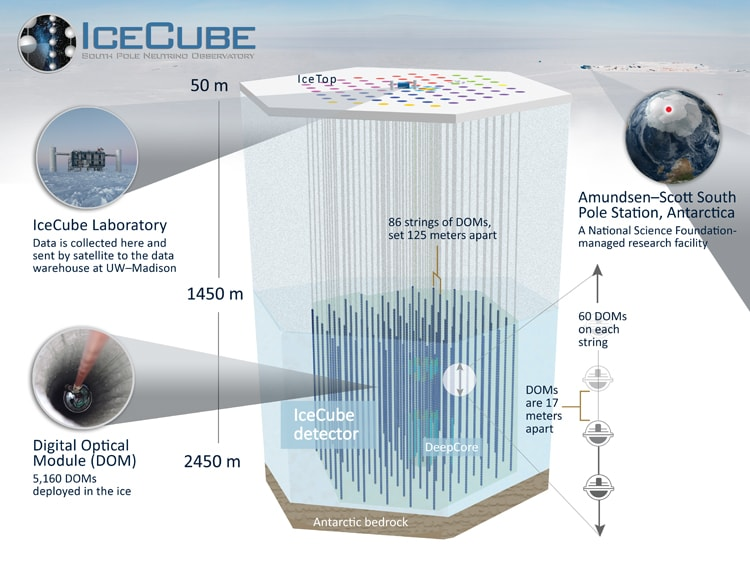
\includegraphics[width=1\textwidth]{graphics/IceCube.jpg}
  \caption{Schematic structure of the IceCube experiment \cite{IceCube}.}
  \label{fig:cube}
\end{figure}

Neutrinos are measured via secondary particles of the charged current
\begin{equation*}
  \nu_l (\bar{\nu}_l) + A \to l^{\mp} + X
\end{equation*}
or the neutral current
\begin{equation*}
  \nu_l + A \to \nu_l + X\,.
\end{equation*}

Due to their high energy loss electrons have a spherical signature of Cherenkov light while muons have a longer signature since their energy loss is much lower.
Tau leptons possess a similar spherical signature as electrons since the life time is very low resulting in a low reach before decaying.
In the neutral current a cascade induced by the secondary hadrons is observed which has also a similar signature as electrons.
Cherenkov light from muons is too weak to be detected but muons interacting with the medium are producing $e^+e^-$ pairs and photons which are resulting in a cascade.
The Cherenkov light of these secondary particles can be measured by the experiment.

\subsection{Measurement of neutrinos with the IceCube experiment}
An analysis method to reject atmospherical muons is to use \textit{starting events}.
In this technique the outer layers of the detector are used as a veto for these atmospherical muons.
All neutrino flavours are taken into account equally.
Therefore the biggest contributions of events come from the neutral current and electron neutrino and tau neutrino via the charged current.
These events have a good energy and a poor angular resolution.
Tracks of muons on the other hand have a poor energy and a good angular resolution as well as a bigger reach.
Planet earth itself can be used as a shield for atmospheric muons since they would be absorbed mostly.
In result muons that come from that side have to be from neutrino interactions.
To separate atmospherical muons from muon neutrinos a cut on the zenith angle can be made.
Since the track reconstruction is not perfect a cut on the zenith angle is just resulting in an improvement of the signal to background ratio from $1\!:\!10^6$ to $1\!:\!10^3$.
To improve the separation from muons and muon neutrinos even further procedures of machine learning are used.
The separation of signal and background is the aim of this analysis.
